% For tracking purposes - this is V3.1SP - APRIL 2009
\documentclass{acm_proc_article-sp}

\usepackage[utf8]{inputenc}
\usepackage[unicode=true,hidelinks]{hyperref}

\begin{document}

\title{An Architecture Pattern for Network Resilient Web Applications}

\numberofauthors{3}
\author{
\alignauthor
Julien Richard-Foy\\
       \affaddr{IRISA}\\
       \affaddr{Université de Rennes, France}\\
       \email{julien.richard-foy@irisa.fr}
\alignauthor
Olivier Barais\\
       \affaddr{IRISA}\\
       \affaddr{Université de Rennes, France}\\
       \email{olivier.barais@irisa.fr}
\alignauthor Jean-Marc Jézéquel\\
       \affaddr{INRIA}\\
       \affaddr{Université de Rennes, France}\\
       \email{jezequel@inria.fr}
}
\date{16 March 2014}

\maketitle
\begin{abstract}
Network resilience is a cross-cutting concern in the development of Web applications. This paper presents a synchronization algorithm and an architecture pattern isolating the network resilience concern.
\end{abstract}

% A category with the (minimum) three required fields
\category{H.4}{Information Systems Applications}{Miscellaneous}
%A category including the fourth, optional field follows...
\category{D.2.8}{Software Engineering}{Metrics}[complexity measures, performance measures]

\terms{Theory}

\keywords{ACM proceedings, \LaTeX, text tagging} % NOT required for Proceedings

\section{Introduction}

The Web is a convenient application platform: no installation or deployment step on clients, collaborative work, support of heterogeneous clients, \textit{etc}. However, Web applications work only as long as the network connection and the server are up. If the network connection or the server is down, Web applications may suffer from inconsistency, freeze or latency, resulting in a bad user experience. With the advent of Internet connected mobile devices (smartphones and tablets) rises the need for a good support of an off-line mode for Web applications.

In this paper, we use the term \textit{resilience} to refer to the ability of a Web application to deliver a good Quality of Experience (QoE) under bad network conditions. The resilience level can vary. For instance, when an application detects a network failure, it can either:

\begin{itemize}
 \item Display an error message informing the user that its last action failed (\textit{e.g.} Trello\footnote{\href{http://www.trello.com}{http://www.trello.com}});
 \item Fallback to a read-only mode (\textit{e.g.} Google Drive\footnote{\href{http://drive.google.com}{http://drive.google.com}});
 \item Store the actions performed by the user and try to synchronize them to the server when the connection is back (\textit{e.g.} Workflowy\footnote{\href{http://www.workflowy.com}{http://www.workflowy.com}}).
\end{itemize}

Achieving resilience can be more or less hard according to the application’s domain. In all cases, resilience is a cross-cutting concern: any action performed by the user may trigger an AJAX call that may fail. To keep delivering a good QoE when the server is unreachable, the application must resite the business logic on the client-side and then synchronize the changes to the server when the connection comes back.

In the particular case of collaborative applications, the synchronization step can be challenging: if two clients concurrently change the same resource, how can the server decide which one wins? The more the number of concurrent actions clients can perform without synchronizing to the server, the higher is the risk to be unable to order them.

Our paper presents an architecture pattern based on event sourcing to achieve resilience in Web applications. Our pattern is agnostic to the whole application architecture, it requires little adaptation for existing applications to use it, it only captures and isolates the client-server synchronization process and allows to deliver a good QoE when the network is down. To resolve synchronization conflicts, our pattern can be mixed with either operational transformation or conflict-free replicated data types approaches.

We implemented our pattern as libraries for both server and client sides and used it to develop several use case applications demonstrating the isolation of the resilience concern. We proved the eventual consistency of our synchronization algorithm.

\section{Related Works}

\subsection{Offline Support}

\subsection{Collaborative Work}

\paragraph{Operational Transformation}

\paragraph{Conflict-free Replicated Data Types}

\subsection{Persistent Resources}

\section{Contribution}

\subsection{Architecture}

\begin{figure*}
\centering
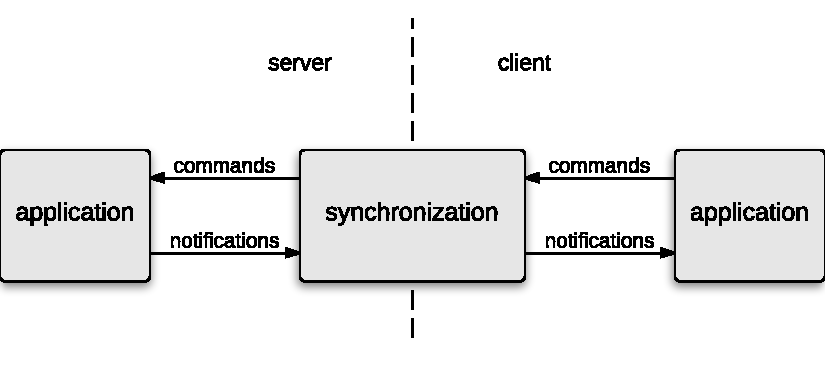
\includegraphics[width=10cm]{arch-overview.pdf}
\label{fig-arch-overview}
\end{figure*}

\begin{figure*}
\centering
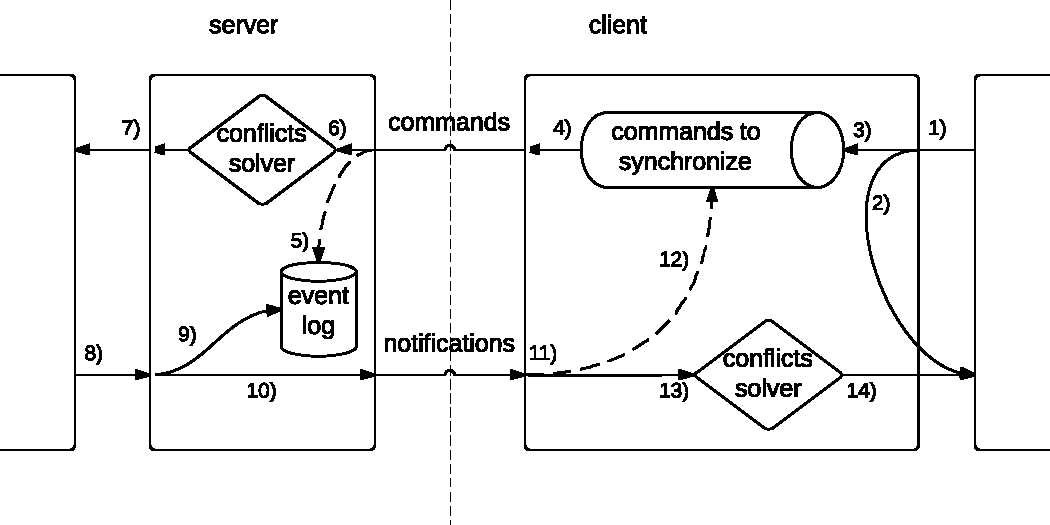
\includegraphics[width=10cm]{arch-detail.pdf}
\end{figure*}


\subsection{Synchronization}

We propose an algorithm to achieve synchronization between clients and server. Web architectures are centralized distributed systems, making it simpler to achieve synchronization than in a completely decentralized system.

Our algorithm uses a logical clock on the server only: each command applied by the server acts as a tick. The clock is used to detect precedence between commands.

The goal of the synchronization algorithm is to provide eventual consistency between all clients.

Each time a client performs an action, the synchronization component assigns it a unique identifier, appends it into a queue and invokes the corresponding logic, defined by the application. If the network connection is up, the synchronization also tries to send the command to the server along with the timestamp of the last known command applied by the server.

When the server receives a synchronization message from a client, consisting of a timestamp of the last known command applied and a command to apply it first checks if the client missed some events and sends them. Then it determines, using the timestamp, the commands that have been applied without being notified to the client, and transforms the commands given in the message according to these missed commands so the effect of their application is intention preserving. The server then applies the transformed commands (by invoking the logic defined by the application), appends them to an event log and associates them a timestamp. Finally, the produced timestamped events are broadcasted to all clients.

When a client receives a notification message, consisting of a timestamp and an event, it checks if the event corresponds to a command in its queue. If that is the case it just removes the corresponding command from the queue, appends the event to a log and sets the timestamp of the last known command applied by the server to the event timestamp. Otherwise (if the event corresponds to a command initiated by another client), the command logic is invoked on the client after having been transformed according to the commands that have been locally applied but not sent to the server, the event is append to a log and the timestamp of the last known command applied by the server is updated.

\section{Validation}

\subsection{Reusable Library}

\subsection{Synchronization Algorithm Eventual Consistency}

\subsection{Limitations}

\subsubsection{Data Loading}

\subsubsection{Notifications Personalization}

\section{Discussion}

\balancecolumns
% That's all folks!
\end{document}
